\input{header_slides}

\begin{document}

\title[Models of urban morphogenesis]{Models of urban morphogenesis to link urban form and function}
\author[J. Raimbault]{J.~Raimbault$^{1,2,3\ast}$\\\medskip
$^{\ast}$\texttt{j.raimbault@ucl.ac.uk}
}

\institute[UCL]{$^{1}$CASA, UCL\\
$^{2}$UPS CNRS 3611 Complex Systems Institute Paris\\
$^{3}$UMR CNRS 8504 G{\'e}ographie-cit{\'e}s
}




\date[15th November 2019]{TQG Debates 2019\\
3.1: Fractals and Multi-fractals\\
November 15th 2019
}

\frame{\maketitle}



% \textbf{Keywords: }\textit{Urban growth; Reaction-diffusion; World urban areas; Model calibration}

%  Understanding drivers of urban growth and land-use change at the metropolitan scale often requires to isolate and estimate stylized processes of urban evolution. Several land-use change and urban growth models for example based on cellular automata have been introduced in the literature, but their lack of generality and need for rich data may become a shortcoming. We propose here to apply and calibrate a simple model of urban growth based on reaction-diffusion processes for population density, providing a rather general insight into world urban areas from simple data. This four-parameter model introduced by \cite{raimbault2018calibration} combines aggregation forces (positive externalities) with dispersal forces (negative externalities) to capture dynamics of urban form. The model was previously only simulated on synthetic initially empty spaces and statically calibrated by comparing the projection of final simulated configurations in a space of urban morphology indicators (Moran index, entropy, average distance, hierarchy) to real measures computed on a fixed-size moving window for Europe. We significantly extend these result by (i) applying the model on the 1000 largest urban areas of the Global Human Settlements database \citep{Florczyk2019ghs}; (ii) proceeding to a calibration on three successive time windows (1975-1990, 1990-2000 and 2000-2015) what provides dynamical values for parameters; (iii) using genetic optimization algorithms to minimise the distance on morphological indicators for each area. The computational cost being high, results are obtained by using the OpenMOLE model exploration software \citep{reuillon2013openmole}, which provides in a transparent way the optimization algorithms and the distribution of calibrations on a computation grid. We obtain therein comparable values for aggregation, diffusion and growth speed parameters on all these areas for the three periods given above. These values can be used for short terms projections, but also high-level policies by situating urban areas in the model phase diagrams and for example comparing them to more or less close phase transition parameter values. We also illustrate possible policy applications by relating estimated parameters to the EDGAR greenhouse gases emission database. This work thus shows how simple models can be useful for global comparisons, which are necessary to contextualize territorial policies.






\section{Introduction}


\sframe{Complex processes of Urban Morphogenesis}{

\centering

% center of Paris
%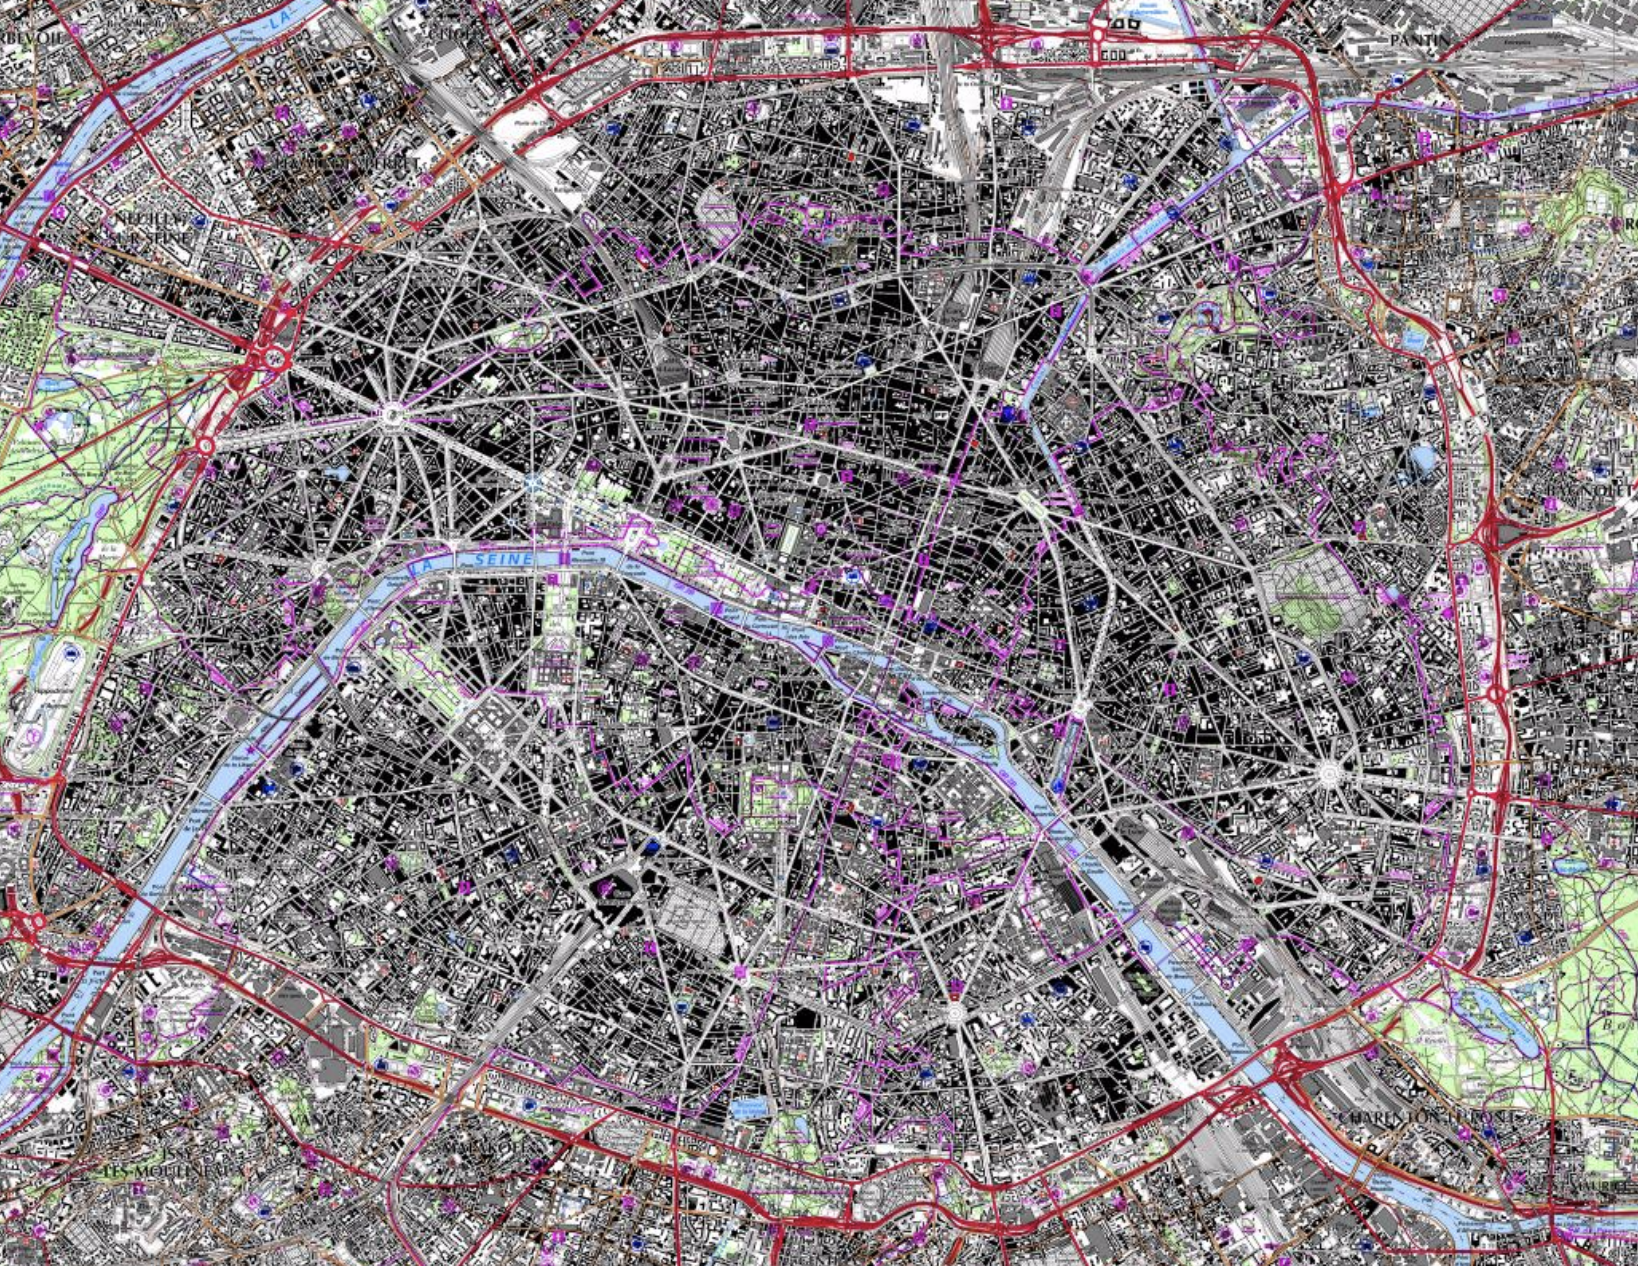
\includegraphics[width=0.88\textwidth]{figures/intro_paname}
%\includegraphics[width=0.9\textwidth]{figures/intro_bp}

\footnotesize\textit{Source: Geoportail}
}





\sframe{Defining Morphogenesis}{

% precise notions and defs

\justify

\textit{Proposition of an interdisciplinary definition}

\bigskip




\textbf{Meta-epistemological framework of imbricated notions:}

Self-organization $\supsetneq$ Morphogenesis $\supsetneq$ Autopoiesis $\supsetneq$ Life


\bigskip

\textbf{Properties:}

\begin{itemize}
\item Architecture links form and function
\item Emergence strength~\cite{bedau2002downward} increases with notion depth, as bifurcations~\cite{thom1974stabilite}
\end{itemize}

\bigskip

\textbf{Definition of Morphogenesis :} \textit{Emergence of the form and the function in a strongly coupled manner, producing an emergent architecture \cite{doursat2012morphogenetic}}



}



\sframe{Which models for Urban Morphogenesis ?}{

% why modeling, exemple of rbd
% -> champ ; difficultés ("verrous". rq : j'aime pas la metaphore du verrou, trop cadrant et suppose que deja construit et qu'il suffit d'ouvrir. demarche epistemo de co-evol des connaissances, ni inductif ni deductif. il faut contruire. horizons d'exploration plus appropriés. rejoint l'idee de faire rentrer dans "cadre analytique" : cases prédéfinies, alors qu'il s'agit au contraire de définir ces cases. -> relire hdr arnaud

\justify

\begin{columns}
\column{0.35\textwidth}
\centering
\includegraphics[width=\textwidth]{figures/intro_RBD_lattice}\\
\footnotesize\textit{Example: a basic hybrid model based on elementary processes for density and network \cite{raimbault2014hybrid}}
\column{0.6\textwidth}
\justify

%\vspace{-1cm}

$\rightarrow$\textit{At the crossroad between Urban Simulation and Artificial Life, few models try to integrate and explain the link between Urban Form and Function}

\medskip

$\rightarrow$\textit{Importance of parcimonious, stylized models: modeling as a tool to understand processes}

\end{columns}

\bigskip

\textbf{Research Objective : } Explore simple models to capture morphogenesis based on abstract representation of urban processes; test their ability to reproduce existing urban systems.



}


\section{Reaction-diffusion model}


\sframe{A simple Reaction-diffusion model}{

% comment Arnaud : reaction-diffusion ?

% model rationale and processes


\justify

$\rightarrow$ Crucial role of the interplay between concentration forces and dispersion forces~\cite{fujita1996economics} in keeping Urban Systems at the border of chaos

\bigskip

$\rightarrow$ Potentiality of aggregation mechanisms (such as Simon model) to produce power laws \cite{dodds2017simon}

\bigskip

$\rightarrow$ Link with Reaction-diffusion approaches in Morphogenesis~\cite{turing1952chemical}

\bigskip

$\rightarrow$ Extension of a DLA-type model introduced by \cite{batty1991generating}, with simple abstract processes of population aggregation and diffusion

\bigskip
\bigskip

{\tiny

Raimbault, J. (2018). Calibration of a density-based model of urban morphogenesis. PloS one, 13(9), e0203516.
}

}

\sframe{Model Formalization}{

% model formalization and indicators

$\rightarrow$ Grid world with cell populations $\left(P_i\left(t\right)\right)_{1\leq i\leq N^2}$.

\bigskip

$\rightarrow$ At each time step:


\begin{enumerate}
\item Population growth with exogenous rate $N_G$, attributed independently to a cell following a preferential attachment of strength $\alpha$
%\begin{equation}
%\Pb{P_i(t+1)=P_i(t)+1|P(t+1)=P(t)+1}=\frac{(P_i(t)/P(t))^{\alpha}}{\sum(P_i(t)/P(t))^{\alpha}}
%\end{equation}
%The attribution being uniformly drawn if all population are equal to 0.
\item Population is diffused $n_d$ times with strength $\beta$
\end{enumerate}

\bigskip

$\rightarrow$ Stopping criterion: fixed maximal population $P_m$.

%To avoid bord effects such as reflecting diffusion waves, border cells diffuse their due proportion outside of the world, implying that the total population at time $t$ is strictly smaller than $N_G\cdot t$.

\bigskip

$\rightarrow$ Output measured by morphological indicators: Moran index, average distance, rank-size hierarchy, entropy.


}


\sframe{Generating Population Distributions}{


% examples : fig 2 of paper

\centering

\includegraphics[height=0.8\textheight]{figures/density_Fig2}

\footnotesize\textit{Examples of generated territorial shapes}

}


\sframe{Model behavior}{

\centering

\includegraphics[width=0.9\textwidth]{figures/density_Fig3}

\footnotesize\textit{Phase transitions of indicators unveiled by exploration of the parameter space (80000 parameter points, 10 repetitions each)}


}




\sframe{Path-dependence and frozen accidents}{

\centering

\includegraphics[width=0.8\textwidth]{figures/density_Fig4}

\footnotesize\textit{Illustration of path-dependence in a simplified one-dimensional version of the model: cell trajectories in time for 9 independent repetitions from the same initial configuration.}


}


\sframe{Empirical Data for Calibration}{

% comments Arnaud : Quel lien avec les slides avant et après ? "Real" : le terme me paraît discutable : données empiriques plutôt ?
%  Décrire les données car ici tu passes directement aux indicateurs

\begin{columns}
\column{0.6\textwidth}
\centering
\includegraphics[width=\textwidth]{figures/density_indics_morpho_discrquantiles}
\column{0.3\textwidth}
\centering
\includegraphics[width=\textwidth]{figures/density_cluster_pca_k5_morpho}\\
\includegraphics[width=\textwidth]{figures/density_cluster_map_k5_morpho}
\end{columns}

\justify

\footnotesize\textit{Computation of morphological indicators on population density data for Europe (shown here on France), morphological classification.}

}



\sframe{Model Calibration}{

\includegraphics[width=0.9\textwidth]{figures/density_synth}

\footnotesize\textit{Brute force calibration by exploring the parameter space. Reproduction of most existing configuration in the morphological sense (here in principal plan).}

}



\sframe{Model Targeted Exploration}{

\centering

\includegraphics[width=0.8\textwidth]{figures/density_Fig6}

\footnotesize\textit{Potentialities of targeted model explorations: here feasible space using Pattern Space Exploration algorithm \cite{10.1371/journal.pone.0138212}.}

}



\section{Co-evolution model}


\sframe{Including more complex processes ?}{

% transition : representation of territories

\textit{Which ontology to include more complex functional properties ?}

\medskip

$\rightarrow$ Territorial systems as the strong coupling between territories and (potential and realized) networks \cite{dupuy1987vers}.

\medskip

$\rightarrow$ Networks convey functional notions of centralities and accessibility, among others; have furthermore proper topological properties.


}



\section{Discussion}



\sframe{Discussion}{

\justify

\vspace{-1cm}

\textbf{Implications}

$\rightarrow$ This rather simple model reproduces most of existing urban forms in Europe for both population distribution and road network : which intrinsic dimension to the urban system and its morphological aspect ?

$\rightarrow$ Ability to reproduce static correlations and a variety of dynamical lagged correlation regimes suggests that the model captures some of the processes of co-evolution

% implications for morphogenesis ?

\bigskip

\textbf{Developments}


$\rightarrow$ Towards a dynamical calibration ? Need of dynamical data

$\rightarrow$ Investigate the link between spatial non-stationarity and non-ergodicity through simulation by the model

$\rightarrow$ Compare network generation in a ``fair'' way (correcting for additional parameters, open question for models of simulation)


}



\sframe{Towards policy applications}{

% more data

\justify

\textbf{More realistic models?}

\medskip

$\rightarrow$ Introducing more concrete ontologies, economic processes \\
\cite{bonin2014modelisation}, qualitative differentiation \cite{bonin2012modele}, governance processes \cite{le2015modeling}

\medskip

$\rightarrow$ Possible bridges with Land-use change models/Land-use Transport models \cite{wegener2004land}, with systems of cities models\\
 \cite{pumain2017urban}

\medskip

\textbf{More data-driven models?}

\medskip

$\rightarrow$ Work in progress: calibration of the reaction-diffusion model on world urban areas with the Global Human Settlements Layer database

\medskip

$\rightarrow$ Link with sustainability indicators: GHG emissions, economics, etc. \cite{raimbault2019multi}

\medskip

$\rightarrow$ Study models on hybrid synthetic data \cite{raimbault2018space}: systematic conclusions for policies



}




\sframe{Conclusion}{


\justify

$\rightarrow$ A novel model of urban morphogenesis at the mesoscopic scale systematically explored: \textbf{need for more coupling and comparison of models.}

\medskip

$\rightarrow$ At the macro scale of the system of cities? \textbf{Need for multi-scale models.}

\medskip

$\rightarrow$ With more refined urban characteristics and other dimensions ? \textbf{Need for more interdisciplinarity.}

\bigskip
\bigskip
\bigskip

\footnotesize{ - Code, data and results available at\\ \texttt{https://github.com/JusteRaimbault/CityNetwork}\\
- Acknowledgments: Thanks to the \textit{European Grid Infrastructure} and its \textit{National Grid Initiatives} (\textit{France-Grilles} in particular) to give the technical support and the infrastructure.

}

}



\section*{Reserve slides}


\sframe{Reserve slides}{

\centering

\Large

\textbf{Reserve Slides}

}






\sframe{Model classification : PDE}{

% derived PDE

The one-dimensional model verifies the PDE :

\begin{equation}\label{eq:pde}
\begin{split}
\delta t \cdot \frac{\partial p}{\partial t} \textrm{ = } \frac{N_G \cdot p^{\alpha}}{P_{\alpha}(t)} \textrm{ + } \frac{\alpha \beta \left(\alpha - 1\right) \delta x^2}{2}\cdot \frac{N_G \cdot p^{\alpha-2}}{P_{\alpha}\left(t\right)} \cdot \left(\frac{\partial p}{\partial x}\right)^2\\
\textrm{ + } \frac{\beta \delta x^2}{2} \cdot \frac{\partial^2 p}{\partial x^2} \cdot\left[ 1 \textrm{ + } \alpha \frac{N_G p^{\alpha - 1}}{P_{\alpha(t)}} \right]
\end{split}
\end{equation}

}


\sframe{Stationary behavior of 1D model}{
\centering
\includegraphics[width=\textwidth]{figures/density_stationary}
}

\sframe{Stationary behavior of 1D model}{
\centering
\includegraphics[width=0.48\textwidth]{figures/density_pmax_alpha}
\includegraphics[width=0.48\textwidth]{figures/density_pmax_logbeta}

}



\sframe{Morphological indicators}{

\begin{enumerate}
\item Rank-size slope $\gamma$, given by $\ln \left( P_{\tilde{i}}/P_0\right) \sim k \textrm{ + } \gamma\cdot \ln \left(\tilde{i}/i_0\right)$ where $\tilde{i}$ are the indexes of the distribution sorted in decreasing order.
\item Entropy of the distribution:
\begin{equation}
\mathcal{E} \textrm{ = } \sum_{i=1}^{M}\frac{P_i}{P}\cdot \ln{\frac{P_i}{P}}
\end{equation}
$\mathcal{E}\textrm{ = }0$ means that all the population is in one cell whereas $\mathcal{E}\textrm{ = }0$ means that the population is uniformly distributed.
\item Spatial-autocorrelation given by Moran index, with simple spatial weights given by $w_{ij} \textrm{ = } 1/d_{ij}$
\[
I \textrm{ = } M \cdot \frac{\sum_{i\neq j} w_{ij} \left(P_i - \bar{P}\right)\cdot\left(P_j - \bar{P}\right)}{\sum_{i\neq j} w_{ij} \sum_{i}{\left( P_i - \bar{P}\right)}^2}
\]
\item Mean distance between individuals
\[
\bar{d} \textrm{ = } \frac{1}{d_M}\cdot \sum_{i<j} \frac{P_i P_j}{P^2} \cdot d_{ij}
\]
where $d_M$ is a normalisation constant
\end{enumerate}



}


\sframe{Model behavior : Convergence}{

Large number of repetitions show good convergence properties

% hist examples

\includegraphics[width=0.5\textwidth]{figures/density_hist_moran}
\includegraphics[width=0.5\textwidth]{figures/density_hist_slope}

}


\sframe{Model behavior}{


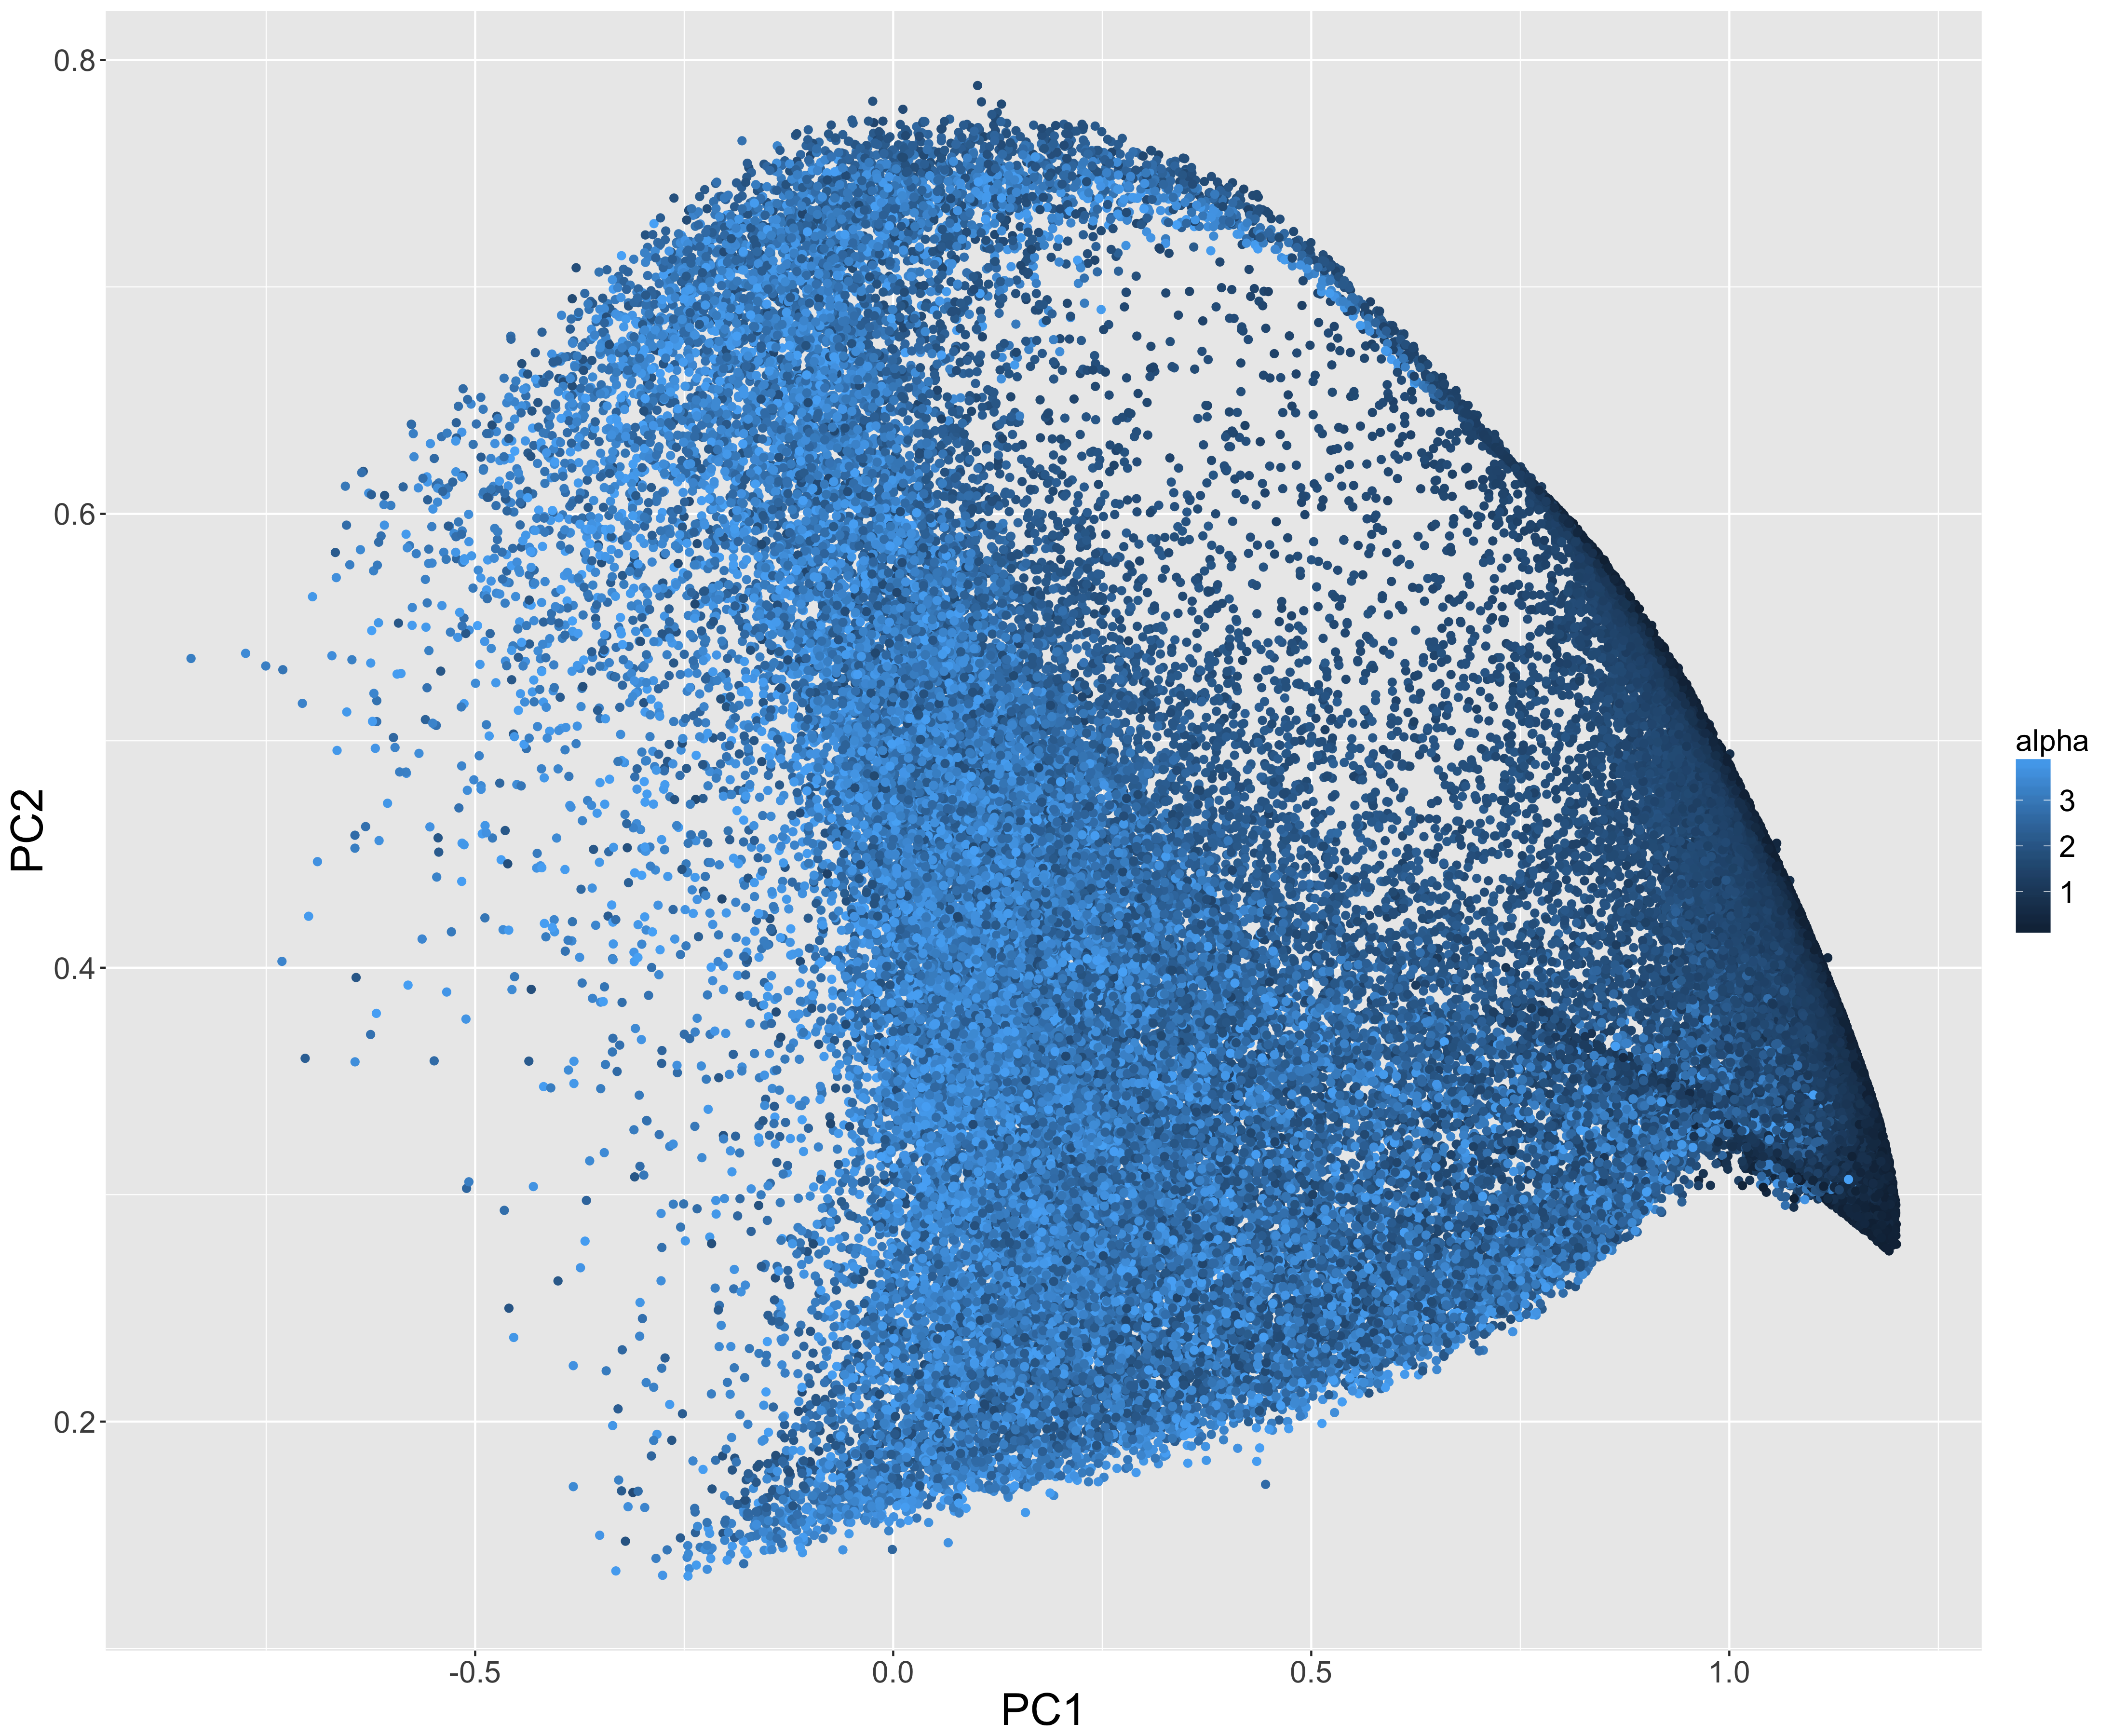
\includegraphics[width=0.5\textwidth]{figures/density_pc_colalpha}
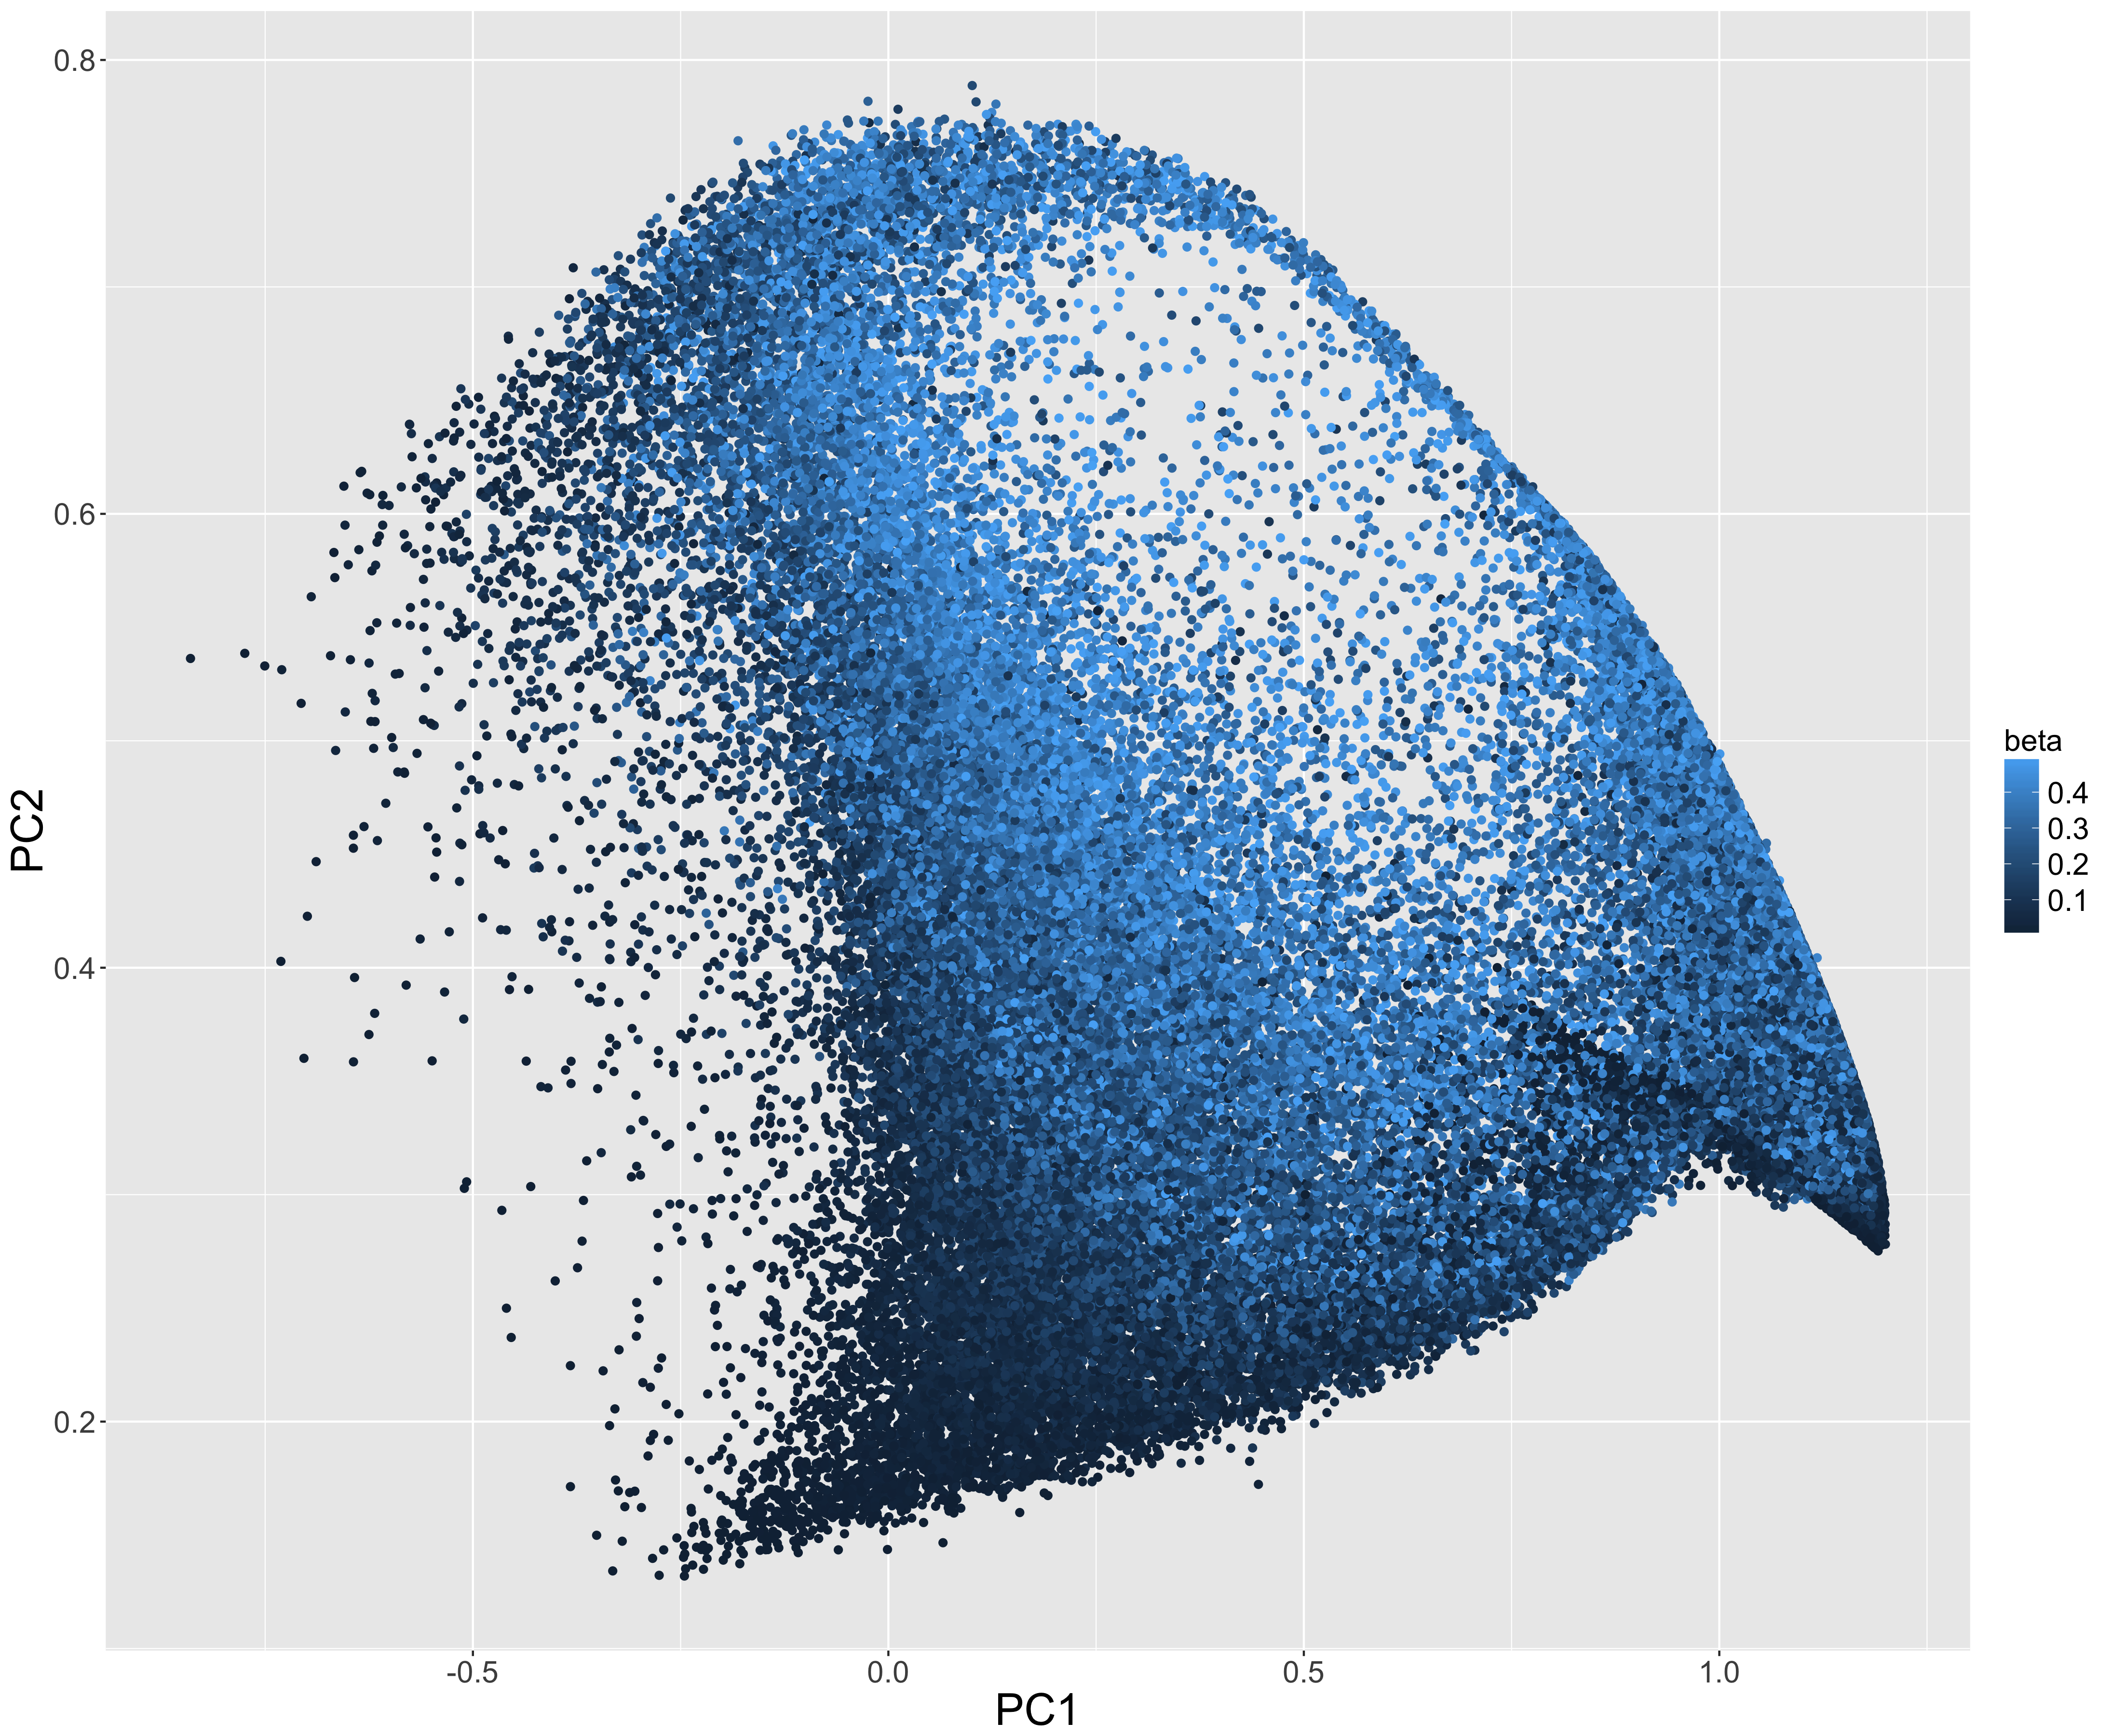
\includegraphics[width=0.5\textwidth]{figures/density_pc_colbeta}

}


\sframe{Empirical indicators computation}{

$\rightarrow$ Eurostat population density raster (100m, simplified at 500m resolution)

\medskip

$\rightarrow$ Overlapping (10km offset) squares of 50km side : equivalent to smoothing, removes window shape effect. Not very sensitive to window size (tested with 30km and 100km)

\medskip

$\rightarrow$ Indicators computed using Fast Fourier Transform Convolution

\medskip

$\rightarrow$ Classification using repeated k-means ; number of clusters taken at transition in clustering coefficient.

}

\sframe{Model calibration: all indicators}{

\centering
\includegraphics[width=0.65\textwidth]{figures/density_scatter}

}




%%%%%%%%%%%%%%%%%%%%%
\begin{frame}[allowframebreaks]
\frametitle{References}
\bibliographystyle{apalike}
\bibliography{biblio}
\end{frame}
%%%%%%%%%%%%%%%%%%%%%%%%%%%%





%\sframe{What is Morphogenesis ? Examples}{

% illustrations : ants, geomorphology, neurons, self-assembly ; ARBOTRON ; paper nature aile avion
% all from netlogo library ? would be nice illustration of generative nature


% remark : do not put classical biological example to show how it has percolated to other fields
%\vspace{-0.3cm}
%\includegraphics[width=\textwidth,height=0.82\textheight]{figures/intro_examples}

%\justify

%\vspace{-0.5cm}

%\footnotesize\textit{Sources (in order by column). Ants, Erosion, Game of Life: NetLogo Library; Arbotron \cite{jun2005formation}; Industrial design \cite{Aage:2017aa}; Swarm chemistry \cite{sayama2007decentralized}}
% sources : ants netlogo ; erosion netlogo ; arbotron 
%  inge : 
%}



\end{document}






